\section{Spark::Sp\-Gpu\-Program Class Reference}
\label{classSpark_1_1SpGpuProgram}\index{Spark::SpGpuProgram@{Spark::SpGpuProgram}}
{\tt \#include $<$Sp\-Gpu\-Program.h$>$}

Inheritance diagram for Spark::Sp\-Gpu\-Program:\begin{figure}[H]
\begin{center}
\leavevmode
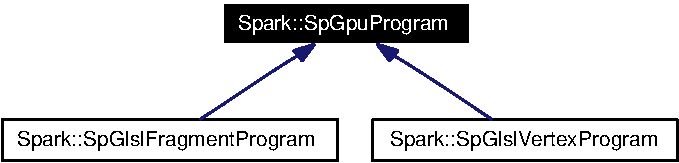
\includegraphics[width=180pt]{classSpark_1_1SpGpuProgram__inherit__graph}
\end{center}
\end{figure}


\subsection{Detailed Description}
Abstract base class for a GPU program. 

Definition at line 33 of file Sp\-Gpu\-Program.h.\subsection*{Public Types}
\begin{CompactItemize}
\item 
enum {\bf Type} \{ {\bf GPU\_\-INVALID\_\-PROGRAM}, 
{\bf GPU\_\-GLSL\_\-VERTEX\_\-PROGRAM}, 
{\bf GPU\_\-GLSL\_\-FRAGMENT\_\-PROGRAM}, 
{\bf GPU\_\-PROGRAM\_\-COUNT}
 \}
\begin{CompactList}\small\item\em Enumerations:. \item\end{CompactList}\end{CompactItemize}
\subsection*{Public Member Functions}
\begin{CompactItemize}
\item 
virtual {\bf $\sim$Sp\-Gpu\-Program} ()
\begin{CompactList}\small\item\em Construction:. \item\end{CompactList}\item 
char $\ast$ {\bf get\-Source} ()
\begin{CompactList}\small\item\em Attributes:. \item\end{CompactList}\item 
void {\bf set\-Source} (const char $\ast$ac\-Sp\-Gpu\-Program)
\item 
unsigned int {\bf get\-Length} ()
\item 
{\bf Sp\-Gpu\-Program::Type} {\bf get\-Type} () const
\item 
void {\bf set\-User\-Data} (const void $\ast$pv\-Data, int i\-Size)
\begin{CompactList}\small\item\em User Data Methods:. \item\end{CompactList}\item 
void {\bf get\-User\-Data} (void $\ast$pv\-Data, int i\-Size) const
\item 
void {\bf set\-State} ()
\begin{CompactList}\small\item\em State Methods:. \item\end{CompactList}\item 
void {\bf reset\-State} ()
\item 
void {\bf enable\-Client\-State} (const char $\ast$ac\-Name)
\item 
void {\bf disable\-Client\-State} (const char $\ast$ac\-Name)
\item 
void {\bf destroy} ()
\item 
virtual bool {\bf set\-Parameter1i} (const char $\ast$ac\-Name, int i\-X)
\begin{CompactList}\small\item\em Parameter Methods:. \item\end{CompactList}\item 
virtual bool {\bf set\-Parameter2i} (const char $\ast$ac\-Name, int i\-X, int i\-Y)
\item 
virtual bool {\bf set\-Parameter3i} (const char $\ast$ac\-Name, int i\-X, int i\-Y, int i\-Z)
\item 
virtual bool {\bf set\-Parameter4i} (const char $\ast$ac\-Name, int i\-X, int i\-Y, int i\-Z, int i\-W)
\item 
virtual bool {\bf set\-Parameter1iv} (const char $\ast$ac\-Name, const float $\ast$af\-Values, int i\-Count=1)
\item 
virtual bool {\bf set\-Parameter2iv} (const char $\ast$ac\-Name, const float $\ast$af\-Values, int i\-Count=1)
\item 
virtual bool {\bf set\-Parameter3iv} (const char $\ast$ac\-Name, const float $\ast$af\-Values, int i\-Count=1)
\item 
virtual bool {\bf set\-Parameter4iv} (const char $\ast$ac\-Name, const float $\ast$af\-Values, int i\-Count=1)
\item 
virtual bool {\bf set\-Parameter1f} (const char $\ast$ac\-Name, float f\-X)
\item 
virtual bool {\bf set\-Parameter2f} (const char $\ast$ac\-Name, float f\-X, float f\-Y)
\item 
virtual bool {\bf set\-Parameter3f} (const char $\ast$ac\-Name, float f\-X, float f\-Y, float f\-Z)
\item 
virtual bool {\bf set\-Parameter4f} (const char $\ast$ac\-Name, float f\-X, float f\-Y, float f\-Z, float f\-W)
\item 
virtual bool {\bf set\-Parameter1fv} (const char $\ast$ac\-Name, const float $\ast$af\-Values, int i\-Count=1)
\item 
virtual bool {\bf set\-Parameter2fv} (const char $\ast$ac\-Name, const float $\ast$af\-Values, int i\-Count=1)
\item 
virtual bool {\bf set\-Parameter3fv} (const char $\ast$ac\-Name, const float $\ast$af\-Values, int i\-Count=1)
\item 
virtual bool {\bf set\-Parameter4fv} (const char $\ast$ac\-Name, const float $\ast$af\-Values, int i\-Count=1)
\item 
virtual bool {\bf set\-Matrix\-Parameter2fv} (const char $\ast$ac\-Name, const float $\ast$af\-Values, int i\-Count=1)
\item 
virtual bool {\bf set\-Matrix\-Parameter3fv} (const char $\ast$ac\-Name, const float $\ast$af\-Values, int i\-Count=1)
\item 
virtual bool {\bf set\-Matrix\-Parameter4fv} (const char $\ast$ac\-Name, const float $\ast$af\-Values, int i\-Count=1)
\end{CompactItemize}
\subsection*{Protected Member Functions}
\begin{CompactItemize}
\item 
{\bf Sp\-Gpu\-Program} ({\bf Sp\-Gpu\-Program::Type} e\-Type=GPU\_\-INVALID\_\-PROGRAM)
\begin{CompactList}\small\item\em Internal Data:. \item\end{CompactList}\item 
{\bf Enable\-Referencing} ()
\end{CompactItemize}
\subsection*{Protected Attributes}
\begin{CompactItemize}
\item 
char $\ast$ {\bf m\_\-ac\-Source}
\item 
char {\bf m\_\-ac\-User\-Data} [8]
\item 
unsigned int {\bf m\_\-ui\-Length}
\item 
{\bf Sp\-Gpu\-Program::Type} {\bf m\_\-e\-Type}
\end{CompactItemize}


\subsection{Member Enumeration Documentation}
\index{Spark::SpGpuProgram@{Spark::Sp\-Gpu\-Program}!Type@{Type}}
\index{Type@{Type}!Spark::SpGpuProgram@{Spark::Sp\-Gpu\-Program}}
\subsubsection{\setlength{\rightskip}{0pt plus 5cm}enum {\bf Spark::Sp\-Gpu\-Program::Type}}\label{classSpark_1_1SpGpuProgram_w4}


Enumerations:. 

\begin{Desc}
\item[Enumeration values: ]\par
\begin{description}
\index{GPU_INVALID_PROGRAM@{GPU\_\-INVALID\_\-PROGRAM}!Spark::SpGpuProgram@{Spark::SpGpuProgram}}\index{Spark::SpGpuProgram@{Spark::SpGpuProgram}!GPU_INVALID_PROGRAM@{GPU\_\-INVALID\_\-PROGRAM}}\item[{\em 
GPU\_\-INVALID\_\-PROGRAM\label{classSpark_1_1SpGpuProgram_w4w0}
}]\index{GPU_GLSL_VERTEX_PROGRAM@{GPU\_\-GLSL\_\-VERTEX\_\-PROGRAM}!Spark::SpGpuProgram@{Spark::SpGpuProgram}}\index{Spark::SpGpuProgram@{Spark::SpGpuProgram}!GPU_GLSL_VERTEX_PROGRAM@{GPU\_\-GLSL\_\-VERTEX\_\-PROGRAM}}\item[{\em 
GPU\_\-GLSL\_\-VERTEX\_\-PROGRAM\label{classSpark_1_1SpGpuProgram_w4w1}
}]\index{GPU_GLSL_FRAGMENT_PROGRAM@{GPU\_\-GLSL\_\-FRAGMENT\_\-PROGRAM}!Spark::SpGpuProgram@{Spark::SpGpuProgram}}\index{Spark::SpGpuProgram@{Spark::SpGpuProgram}!GPU_GLSL_FRAGMENT_PROGRAM@{GPU\_\-GLSL\_\-FRAGMENT\_\-PROGRAM}}\item[{\em 
GPU\_\-GLSL\_\-FRAGMENT\_\-PROGRAM\label{classSpark_1_1SpGpuProgram_w4w2}
}]\index{GPU_PROGRAM_COUNT@{GPU\_\-PROGRAM\_\-COUNT}!Spark::SpGpuProgram@{Spark::SpGpuProgram}}\index{Spark::SpGpuProgram@{Spark::SpGpuProgram}!GPU_PROGRAM_COUNT@{GPU\_\-PROGRAM\_\-COUNT}}\item[{\em 
GPU\_\-PROGRAM\_\-COUNT\label{classSpark_1_1SpGpuProgram_w4w3}
}]\end{description}
\end{Desc}

Definition at line 40 of file Sp\-Gpu\-Program.h.

\subsection{Constructor \& Destructor Documentation}
\index{Spark::SpGpuProgram@{Spark::Sp\-Gpu\-Program}!~SpGpuProgram@{$\sim$SpGpuProgram}}
\index{~SpGpuProgram@{$\sim$SpGpuProgram}!Spark::SpGpuProgram@{Spark::Sp\-Gpu\-Program}}
\subsubsection{\setlength{\rightskip}{0pt plus 5cm}Sp\-Gpu\-Program::$\sim${\bf Sp\-Gpu\-Program} ()\hspace{0.3cm}{\tt  [virtual]}}\label{classSpark_1_1SpGpuProgram_a0}


Construction:. 

Definition at line 16 of file Sp\-Gpu\-Program.cpp.

References m\_\-ac\-Source.\index{Spark::SpGpuProgram@{Spark::Sp\-Gpu\-Program}!SpGpuProgram@{SpGpuProgram}}
\index{SpGpuProgram@{SpGpuProgram}!Spark::SpGpuProgram@{Spark::Sp\-Gpu\-Program}}
\subsubsection{\setlength{\rightskip}{0pt plus 5cm}Sp\-Gpu\-Program::Sp\-Gpu\-Program ({\bf Sp\-Gpu\-Program::Type} {\em e\-Type} = {\tt GPU\_\-INVALID\_\-PROGRAM})\hspace{0.3cm}{\tt  [protected]}}\label{classSpark_1_1SpGpuProgram_b0}


Internal Data:. 

Definition at line 8 of file Sp\-Gpu\-Program.cpp.

References m\_\-ac\-Source, m\_\-ac\-User\-Data, and m\_\-ui\-Length.

\subsection{Member Function Documentation}
\index{Spark::SpGpuProgram@{Spark::Sp\-Gpu\-Program}!destroy@{destroy}}
\index{destroy@{destroy}!Spark::SpGpuProgram@{Spark::Sp\-Gpu\-Program}}
\subsubsection{\setlength{\rightskip}{0pt plus 5cm}void Spark::Sp\-Gpu\-Program::destroy ()}\label{classSpark_1_1SpGpuProgram_a11}


\index{Spark::SpGpuProgram@{Spark::Sp\-Gpu\-Program}!disableClientState@{disableClientState}}
\index{disableClientState@{disableClientState}!Spark::SpGpuProgram@{Spark::Sp\-Gpu\-Program}}
\subsubsection{\setlength{\rightskip}{0pt plus 5cm}void Spark::Sp\-Gpu\-Program::disable\-Client\-State (const char $\ast$ {\em ac\-Name})}\label{classSpark_1_1SpGpuProgram_a10}


\index{Spark::SpGpuProgram@{Spark::Sp\-Gpu\-Program}!enableClientState@{enableClientState}}
\index{enableClientState@{enableClientState}!Spark::SpGpuProgram@{Spark::Sp\-Gpu\-Program}}
\subsubsection{\setlength{\rightskip}{0pt plus 5cm}void Spark::Sp\-Gpu\-Program::enable\-Client\-State (const char $\ast$ {\em ac\-Name})}\label{classSpark_1_1SpGpuProgram_a9}


\index{Spark::SpGpuProgram@{Spark::Sp\-Gpu\-Program}!EnableReferencing@{EnableReferencing}}
\index{EnableReferencing@{EnableReferencing}!Spark::SpGpuProgram@{Spark::Sp\-Gpu\-Program}}
\subsubsection{\setlength{\rightskip}{0pt plus 5cm}Spark::Sp\-Gpu\-Program::Enable\-Referencing ()\hspace{0.3cm}{\tt  [protected]}}\label{classSpark_1_1SpGpuProgram_b1}


\index{Spark::SpGpuProgram@{Spark::Sp\-Gpu\-Program}!getLength@{getLength}}
\index{getLength@{getLength}!Spark::SpGpuProgram@{Spark::Sp\-Gpu\-Program}}
\subsubsection{\setlength{\rightskip}{0pt plus 5cm}unsigned int Spark::Sp\-Gpu\-Program::get\-Length ()\hspace{0.3cm}{\tt  [inline]}}\label{classSpark_1_1SpGpuProgram_a3}


Definition at line 129 of file Sp\-Gpu\-Program.h.

Referenced by Spark::Sp\-Glsl\-Manager::compile().\index{Spark::SpGpuProgram@{Spark::Sp\-Gpu\-Program}!getSource@{getSource}}
\index{getSource@{getSource}!Spark::SpGpuProgram@{Spark::Sp\-Gpu\-Program}}
\subsubsection{\setlength{\rightskip}{0pt plus 5cm}char $\ast$ Spark::Sp\-Gpu\-Program::get\-Source ()\hspace{0.3cm}{\tt  [inline]}}\label{classSpark_1_1SpGpuProgram_a1}


Attributes:. 

Definition at line 124 of file Sp\-Gpu\-Program.h.

References Spark::Sp\-Gpu\-Program\-Ptr.

Referenced by Spark::Sp\-Glsl\-Manager::compile().\index{Spark::SpGpuProgram@{Spark::Sp\-Gpu\-Program}!getType@{getType}}
\index{getType@{getType}!Spark::SpGpuProgram@{Spark::Sp\-Gpu\-Program}}
\subsubsection{\setlength{\rightskip}{0pt plus 5cm}{\bf Sp\-Gpu\-Program::Type} Spark::Sp\-Gpu\-Program::get\-Type () const\hspace{0.3cm}{\tt  [inline]}}\label{classSpark_1_1SpGpuProgram_a4}


Definition at line 134 of file Sp\-Gpu\-Program.h.

Referenced by Spark::Sp\-Glsl\-Manager::bind(), Spark::Sp\-Glsl\-Manager::compile(), Spark::Sp\-Glsl\-Manager::enable(), and Spark::Sp\-Glsl\-Manager::is\-Supported().\index{Spark::SpGpuProgram@{Spark::Sp\-Gpu\-Program}!getUserData@{getUserData}}
\index{getUserData@{getUserData}!Spark::SpGpuProgram@{Spark::Sp\-Gpu\-Program}}
\subsubsection{\setlength{\rightskip}{0pt plus 5cm}void Spark::Sp\-Gpu\-Program::get\-User\-Data (void $\ast$ {\em pv\-Data}, int {\em i\-Size}) const\hspace{0.3cm}{\tt  [inline]}}\label{classSpark_1_1SpGpuProgram_a6}


Definition at line 144 of file Sp\-Gpu\-Program.h.

Referenced by Spark::Sp\-Glsl\-Manager::bind(), Spark::Sp\-Glsl\-Manager::enable(), Spark::Sp\-Glsl\-Vertex\-Program::get\-Parameter\-Register(), Spark::Sp\-Glsl\-Fragment\-Program::get\-Parameter\-Register(), and Spark::Sp\-Glsl\-Manager::release().\index{Spark::SpGpuProgram@{Spark::Sp\-Gpu\-Program}!resetState@{resetState}}
\index{resetState@{resetState}!Spark::SpGpuProgram@{Spark::Sp\-Gpu\-Program}}
\subsubsection{\setlength{\rightskip}{0pt plus 5cm}void Spark::Sp\-Gpu\-Program::reset\-State ()}\label{classSpark_1_1SpGpuProgram_a8}


\index{Spark::SpGpuProgram@{Spark::Sp\-Gpu\-Program}!setMatrixParameter2fv@{setMatrixParameter2fv}}
\index{setMatrixParameter2fv@{setMatrixParameter2fv}!Spark::SpGpuProgram@{Spark::Sp\-Gpu\-Program}}
\subsubsection{\setlength{\rightskip}{0pt plus 5cm}bool Sp\-Gpu\-Program::set\-Matrix\-Parameter2fv (const char $\ast$ {\em ac\-Name}, const float $\ast$ {\em af\-Values}, int {\em i\-Count} = {\tt 1})\hspace{0.3cm}{\tt  [virtual]}}\label{classSpark_1_1SpGpuProgram_a28}




Reimplemented in {\bf Spark::Sp\-Glsl\-Fragment\-Program} {\rm (p.\,\pageref{classSpark_1_1SpGlslFragmentProgram_a17})}, and {\bf Spark::Sp\-Glsl\-Vertex\-Program} {\rm (p.\,\pageref{classSpark_1_1SpGlslVertexProgram_a17})}.

Definition at line 128 of file Sp\-Gpu\-Program.cpp.\index{Spark::SpGpuProgram@{Spark::Sp\-Gpu\-Program}!setMatrixParameter3fv@{setMatrixParameter3fv}}
\index{setMatrixParameter3fv@{setMatrixParameter3fv}!Spark::SpGpuProgram@{Spark::Sp\-Gpu\-Program}}
\subsubsection{\setlength{\rightskip}{0pt plus 5cm}bool Sp\-Gpu\-Program::set\-Matrix\-Parameter3fv (const char $\ast$ {\em ac\-Name}, const float $\ast$ {\em af\-Values}, int {\em i\-Count} = {\tt 1})\hspace{0.3cm}{\tt  [virtual]}}\label{classSpark_1_1SpGpuProgram_a29}




Reimplemented in {\bf Spark::Sp\-Glsl\-Fragment\-Program} {\rm (p.\,\pageref{classSpark_1_1SpGlslFragmentProgram_a18})}, and {\bf Spark::Sp\-Glsl\-Vertex\-Program} {\rm (p.\,\pageref{classSpark_1_1SpGlslVertexProgram_a18})}.

Definition at line 134 of file Sp\-Gpu\-Program.cpp.\index{Spark::SpGpuProgram@{Spark::Sp\-Gpu\-Program}!setMatrixParameter4fv@{setMatrixParameter4fv}}
\index{setMatrixParameter4fv@{setMatrixParameter4fv}!Spark::SpGpuProgram@{Spark::Sp\-Gpu\-Program}}
\subsubsection{\setlength{\rightskip}{0pt plus 5cm}bool Sp\-Gpu\-Program::set\-Matrix\-Parameter4fv (const char $\ast$ {\em ac\-Name}, const float $\ast$ {\em af\-Values}, int {\em i\-Count} = {\tt 1})\hspace{0.3cm}{\tt  [virtual]}}\label{classSpark_1_1SpGpuProgram_a30}




Reimplemented in {\bf Spark::Sp\-Glsl\-Fragment\-Program} {\rm (p.\,\pageref{classSpark_1_1SpGlslFragmentProgram_a19})}, and {\bf Spark::Sp\-Glsl\-Vertex\-Program} {\rm (p.\,\pageref{classSpark_1_1SpGlslVertexProgram_a19})}.

Definition at line 140 of file Sp\-Gpu\-Program.cpp.\index{Spark::SpGpuProgram@{Spark::Sp\-Gpu\-Program}!setParameter1f@{setParameter1f}}
\index{setParameter1f@{setParameter1f}!Spark::SpGpuProgram@{Spark::Sp\-Gpu\-Program}}
\subsubsection{\setlength{\rightskip}{0pt plus 5cm}bool Sp\-Gpu\-Program::set\-Parameter1f (const char $\ast$ {\em ac\-Name}, float {\em f\-X})\hspace{0.3cm}{\tt  [virtual]}}\label{classSpark_1_1SpGpuProgram_a20}




Reimplemented in {\bf Spark::Sp\-Glsl\-Fragment\-Program} {\rm (p.\,\pageref{classSpark_1_1SpGlslFragmentProgram_a9})}, and {\bf Spark::Sp\-Glsl\-Vertex\-Program} {\rm (p.\,\pageref{classSpark_1_1SpGlslVertexProgram_a9})}.

Definition at line 80 of file Sp\-Gpu\-Program.cpp.\index{Spark::SpGpuProgram@{Spark::Sp\-Gpu\-Program}!setParameter1fv@{setParameter1fv}}
\index{setParameter1fv@{setParameter1fv}!Spark::SpGpuProgram@{Spark::Sp\-Gpu\-Program}}
\subsubsection{\setlength{\rightskip}{0pt plus 5cm}bool Sp\-Gpu\-Program::set\-Parameter1fv (const char $\ast$ {\em ac\-Name}, const float $\ast$ {\em af\-Values}, int {\em i\-Count} = {\tt 1})\hspace{0.3cm}{\tt  [virtual]}}\label{classSpark_1_1SpGpuProgram_a24}




Reimplemented in {\bf Spark::Sp\-Glsl\-Fragment\-Program} {\rm (p.\,\pageref{classSpark_1_1SpGlslFragmentProgram_a13})}, and {\bf Spark::Sp\-Glsl\-Vertex\-Program} {\rm (p.\,\pageref{classSpark_1_1SpGlslVertexProgram_a13})}.

Definition at line 104 of file Sp\-Gpu\-Program.cpp.\index{Spark::SpGpuProgram@{Spark::Sp\-Gpu\-Program}!setParameter1i@{setParameter1i}}
\index{setParameter1i@{setParameter1i}!Spark::SpGpuProgram@{Spark::Sp\-Gpu\-Program}}
\subsubsection{\setlength{\rightskip}{0pt plus 5cm}bool Sp\-Gpu\-Program::set\-Parameter1i (const char $\ast$ {\em ac\-Name}, int {\em i\-X})\hspace{0.3cm}{\tt  [virtual]}}\label{classSpark_1_1SpGpuProgram_a12}


Parameter Methods:. 



Reimplemented in {\bf Spark::Sp\-Glsl\-Fragment\-Program} {\rm (p.\,\pageref{classSpark_1_1SpGlslFragmentProgram_a1})}, and {\bf Spark::Sp\-Glsl\-Vertex\-Program} {\rm (p.\,\pageref{classSpark_1_1SpGlslVertexProgram_a1})}.

Definition at line 32 of file Sp\-Gpu\-Program.cpp.\index{Spark::SpGpuProgram@{Spark::Sp\-Gpu\-Program}!setParameter1iv@{setParameter1iv}}
\index{setParameter1iv@{setParameter1iv}!Spark::SpGpuProgram@{Spark::Sp\-Gpu\-Program}}
\subsubsection{\setlength{\rightskip}{0pt plus 5cm}bool Sp\-Gpu\-Program::set\-Parameter1iv (const char $\ast$ {\em ac\-Name}, const float $\ast$ {\em af\-Values}, int {\em i\-Count} = {\tt 1})\hspace{0.3cm}{\tt  [virtual]}}\label{classSpark_1_1SpGpuProgram_a16}


Definition at line 56 of file Sp\-Gpu\-Program.cpp.\index{Spark::SpGpuProgram@{Spark::Sp\-Gpu\-Program}!setParameter2f@{setParameter2f}}
\index{setParameter2f@{setParameter2f}!Spark::SpGpuProgram@{Spark::Sp\-Gpu\-Program}}
\subsubsection{\setlength{\rightskip}{0pt plus 5cm}bool Sp\-Gpu\-Program::set\-Parameter2f (const char $\ast$ {\em ac\-Name}, float {\em f\-X}, float {\em f\-Y})\hspace{0.3cm}{\tt  [virtual]}}\label{classSpark_1_1SpGpuProgram_a21}




Reimplemented in {\bf Spark::Sp\-Glsl\-Fragment\-Program} {\rm (p.\,\pageref{classSpark_1_1SpGlslFragmentProgram_a10})}, and {\bf Spark::Sp\-Glsl\-Vertex\-Program} {\rm (p.\,\pageref{classSpark_1_1SpGlslVertexProgram_a10})}.

Definition at line 86 of file Sp\-Gpu\-Program.cpp.\index{Spark::SpGpuProgram@{Spark::Sp\-Gpu\-Program}!setParameter2fv@{setParameter2fv}}
\index{setParameter2fv@{setParameter2fv}!Spark::SpGpuProgram@{Spark::Sp\-Gpu\-Program}}
\subsubsection{\setlength{\rightskip}{0pt plus 5cm}bool Sp\-Gpu\-Program::set\-Parameter2fv (const char $\ast$ {\em ac\-Name}, const float $\ast$ {\em af\-Values}, int {\em i\-Count} = {\tt 1})\hspace{0.3cm}{\tt  [virtual]}}\label{classSpark_1_1SpGpuProgram_a25}




Reimplemented in {\bf Spark::Sp\-Glsl\-Fragment\-Program} {\rm (p.\,\pageref{classSpark_1_1SpGlslFragmentProgram_a14})}, and {\bf Spark::Sp\-Glsl\-Vertex\-Program} {\rm (p.\,\pageref{classSpark_1_1SpGlslVertexProgram_a14})}.

Definition at line 110 of file Sp\-Gpu\-Program.cpp.\index{Spark::SpGpuProgram@{Spark::Sp\-Gpu\-Program}!setParameter2i@{setParameter2i}}
\index{setParameter2i@{setParameter2i}!Spark::SpGpuProgram@{Spark::Sp\-Gpu\-Program}}
\subsubsection{\setlength{\rightskip}{0pt plus 5cm}bool Sp\-Gpu\-Program::set\-Parameter2i (const char $\ast$ {\em ac\-Name}, int {\em i\-X}, int {\em i\-Y})\hspace{0.3cm}{\tt  [virtual]}}\label{classSpark_1_1SpGpuProgram_a13}




Reimplemented in {\bf Spark::Sp\-Glsl\-Fragment\-Program} {\rm (p.\,\pageref{classSpark_1_1SpGlslFragmentProgram_a2})}, and {\bf Spark::Sp\-Glsl\-Vertex\-Program} {\rm (p.\,\pageref{classSpark_1_1SpGlslVertexProgram_a2})}.

Definition at line 38 of file Sp\-Gpu\-Program.cpp.\index{Spark::SpGpuProgram@{Spark::Sp\-Gpu\-Program}!setParameter2iv@{setParameter2iv}}
\index{setParameter2iv@{setParameter2iv}!Spark::SpGpuProgram@{Spark::Sp\-Gpu\-Program}}
\subsubsection{\setlength{\rightskip}{0pt plus 5cm}bool Sp\-Gpu\-Program::set\-Parameter2iv (const char $\ast$ {\em ac\-Name}, const float $\ast$ {\em af\-Values}, int {\em i\-Count} = {\tt 1})\hspace{0.3cm}{\tt  [virtual]}}\label{classSpark_1_1SpGpuProgram_a17}


Definition at line 62 of file Sp\-Gpu\-Program.cpp.\index{Spark::SpGpuProgram@{Spark::Sp\-Gpu\-Program}!setParameter3f@{setParameter3f}}
\index{setParameter3f@{setParameter3f}!Spark::SpGpuProgram@{Spark::Sp\-Gpu\-Program}}
\subsubsection{\setlength{\rightskip}{0pt plus 5cm}bool Sp\-Gpu\-Program::set\-Parameter3f (const char $\ast$ {\em ac\-Name}, float {\em f\-X}, float {\em f\-Y}, float {\em f\-Z})\hspace{0.3cm}{\tt  [virtual]}}\label{classSpark_1_1SpGpuProgram_a22}




Reimplemented in {\bf Spark::Sp\-Glsl\-Fragment\-Program} {\rm (p.\,\pageref{classSpark_1_1SpGlslFragmentProgram_a11})}, and {\bf Spark::Sp\-Glsl\-Vertex\-Program} {\rm (p.\,\pageref{classSpark_1_1SpGlslVertexProgram_a11})}.

Definition at line 92 of file Sp\-Gpu\-Program.cpp.\index{Spark::SpGpuProgram@{Spark::Sp\-Gpu\-Program}!setParameter3fv@{setParameter3fv}}
\index{setParameter3fv@{setParameter3fv}!Spark::SpGpuProgram@{Spark::Sp\-Gpu\-Program}}
\subsubsection{\setlength{\rightskip}{0pt plus 5cm}bool Sp\-Gpu\-Program::set\-Parameter3fv (const char $\ast$ {\em ac\-Name}, const float $\ast$ {\em af\-Values}, int {\em i\-Count} = {\tt 1})\hspace{0.3cm}{\tt  [virtual]}}\label{classSpark_1_1SpGpuProgram_a26}




Reimplemented in {\bf Spark::Sp\-Glsl\-Fragment\-Program} {\rm (p.\,\pageref{classSpark_1_1SpGlslFragmentProgram_a15})}, and {\bf Spark::Sp\-Glsl\-Vertex\-Program} {\rm (p.\,\pageref{classSpark_1_1SpGlslVertexProgram_a15})}.

Definition at line 116 of file Sp\-Gpu\-Program.cpp.\index{Spark::SpGpuProgram@{Spark::Sp\-Gpu\-Program}!setParameter3i@{setParameter3i}}
\index{setParameter3i@{setParameter3i}!Spark::SpGpuProgram@{Spark::Sp\-Gpu\-Program}}
\subsubsection{\setlength{\rightskip}{0pt plus 5cm}bool Sp\-Gpu\-Program::set\-Parameter3i (const char $\ast$ {\em ac\-Name}, int {\em i\-X}, int {\em i\-Y}, int {\em i\-Z})\hspace{0.3cm}{\tt  [virtual]}}\label{classSpark_1_1SpGpuProgram_a14}




Reimplemented in {\bf Spark::Sp\-Glsl\-Fragment\-Program} {\rm (p.\,\pageref{classSpark_1_1SpGlslFragmentProgram_a3})}, and {\bf Spark::Sp\-Glsl\-Vertex\-Program} {\rm (p.\,\pageref{classSpark_1_1SpGlslVertexProgram_a3})}.

Definition at line 44 of file Sp\-Gpu\-Program.cpp.\index{Spark::SpGpuProgram@{Spark::Sp\-Gpu\-Program}!setParameter3iv@{setParameter3iv}}
\index{setParameter3iv@{setParameter3iv}!Spark::SpGpuProgram@{Spark::Sp\-Gpu\-Program}}
\subsubsection{\setlength{\rightskip}{0pt plus 5cm}bool Sp\-Gpu\-Program::set\-Parameter3iv (const char $\ast$ {\em ac\-Name}, const float $\ast$ {\em af\-Values}, int {\em i\-Count} = {\tt 1})\hspace{0.3cm}{\tt  [virtual]}}\label{classSpark_1_1SpGpuProgram_a18}


Definition at line 68 of file Sp\-Gpu\-Program.cpp.\index{Spark::SpGpuProgram@{Spark::Sp\-Gpu\-Program}!setParameter4f@{setParameter4f}}
\index{setParameter4f@{setParameter4f}!Spark::SpGpuProgram@{Spark::Sp\-Gpu\-Program}}
\subsubsection{\setlength{\rightskip}{0pt plus 5cm}bool Sp\-Gpu\-Program::set\-Parameter4f (const char $\ast$ {\em ac\-Name}, float {\em f\-X}, float {\em f\-Y}, float {\em f\-Z}, float {\em f\-W})\hspace{0.3cm}{\tt  [virtual]}}\label{classSpark_1_1SpGpuProgram_a23}




Reimplemented in {\bf Spark::Sp\-Glsl\-Fragment\-Program} {\rm (p.\,\pageref{classSpark_1_1SpGlslFragmentProgram_a12})}, and {\bf Spark::Sp\-Glsl\-Vertex\-Program} {\rm (p.\,\pageref{classSpark_1_1SpGlslVertexProgram_a12})}.

Definition at line 98 of file Sp\-Gpu\-Program.cpp.\index{Spark::SpGpuProgram@{Spark::Sp\-Gpu\-Program}!setParameter4fv@{setParameter4fv}}
\index{setParameter4fv@{setParameter4fv}!Spark::SpGpuProgram@{Spark::Sp\-Gpu\-Program}}
\subsubsection{\setlength{\rightskip}{0pt plus 5cm}bool Sp\-Gpu\-Program::set\-Parameter4fv (const char $\ast$ {\em ac\-Name}, const float $\ast$ {\em af\-Values}, int {\em i\-Count} = {\tt 1})\hspace{0.3cm}{\tt  [virtual]}}\label{classSpark_1_1SpGpuProgram_a27}




Reimplemented in {\bf Spark::Sp\-Glsl\-Fragment\-Program} {\rm (p.\,\pageref{classSpark_1_1SpGlslFragmentProgram_a16})}, and {\bf Spark::Sp\-Glsl\-Vertex\-Program} {\rm (p.\,\pageref{classSpark_1_1SpGlslVertexProgram_a16})}.

Definition at line 122 of file Sp\-Gpu\-Program.cpp.\index{Spark::SpGpuProgram@{Spark::Sp\-Gpu\-Program}!setParameter4i@{setParameter4i}}
\index{setParameter4i@{setParameter4i}!Spark::SpGpuProgram@{Spark::Sp\-Gpu\-Program}}
\subsubsection{\setlength{\rightskip}{0pt plus 5cm}bool Sp\-Gpu\-Program::set\-Parameter4i (const char $\ast$ {\em ac\-Name}, int {\em i\-X}, int {\em i\-Y}, int {\em i\-Z}, int {\em i\-W})\hspace{0.3cm}{\tt  [virtual]}}\label{classSpark_1_1SpGpuProgram_a15}




Reimplemented in {\bf Spark::Sp\-Glsl\-Fragment\-Program} {\rm (p.\,\pageref{classSpark_1_1SpGlslFragmentProgram_a4})}, and {\bf Spark::Sp\-Glsl\-Vertex\-Program} {\rm (p.\,\pageref{classSpark_1_1SpGlslVertexProgram_a4})}.

Definition at line 50 of file Sp\-Gpu\-Program.cpp.\index{Spark::SpGpuProgram@{Spark::Sp\-Gpu\-Program}!setParameter4iv@{setParameter4iv}}
\index{setParameter4iv@{setParameter4iv}!Spark::SpGpuProgram@{Spark::Sp\-Gpu\-Program}}
\subsubsection{\setlength{\rightskip}{0pt plus 5cm}bool Sp\-Gpu\-Program::set\-Parameter4iv (const char $\ast$ {\em ac\-Name}, const float $\ast$ {\em af\-Values}, int {\em i\-Count} = {\tt 1})\hspace{0.3cm}{\tt  [virtual]}}\label{classSpark_1_1SpGpuProgram_a19}


Definition at line 74 of file Sp\-Gpu\-Program.cpp.\index{Spark::SpGpuProgram@{Spark::Sp\-Gpu\-Program}!setSource@{setSource}}
\index{setSource@{setSource}!Spark::SpGpuProgram@{Spark::Sp\-Gpu\-Program}}
\subsubsection{\setlength{\rightskip}{0pt plus 5cm}void Sp\-Gpu\-Program::set\-Source (const char $\ast$ {\em ac\-Sp\-Gpu\-Program})}\label{classSpark_1_1SpGpuProgram_a2}


Definition at line 21 of file Sp\-Gpu\-Program.cpp.

References m\_\-ac\-Source, and m\_\-ui\-Length.

Referenced by Spark::Sp\-Glsl\-Fragment\-Program::Sp\-Glsl\-Fragment\-Program(), and Spark::Sp\-Glsl\-Vertex\-Program::Sp\-Glsl\-Vertex\-Program().\index{Spark::SpGpuProgram@{Spark::Sp\-Gpu\-Program}!setState@{setState}}
\index{setState@{setState}!Spark::SpGpuProgram@{Spark::Sp\-Gpu\-Program}}
\subsubsection{\setlength{\rightskip}{0pt plus 5cm}void Spark::Sp\-Gpu\-Program::set\-State ()}\label{classSpark_1_1SpGpuProgram_a7}


State Methods:. 

\index{Spark::SpGpuProgram@{Spark::Sp\-Gpu\-Program}!setUserData@{setUserData}}
\index{setUserData@{setUserData}!Spark::SpGpuProgram@{Spark::Sp\-Gpu\-Program}}
\subsubsection{\setlength{\rightskip}{0pt plus 5cm}void Spark::Sp\-Gpu\-Program::set\-User\-Data (const void $\ast$ {\em pv\-Data}, int {\em i\-Size})\hspace{0.3cm}{\tt  [inline]}}\label{classSpark_1_1SpGpuProgram_a5}


User Data Methods:. 

Definition at line 139 of file Sp\-Gpu\-Program.h.

Referenced by Spark::Sp\-Glsl\-Manager::compile(), and Spark::Sp\-Glsl\-Manager::release().

\subsection{Member Data Documentation}
\index{Spark::SpGpuProgram@{Spark::Sp\-Gpu\-Program}!m_acSource@{m\_\-acSource}}
\index{m_acSource@{m\_\-acSource}!Spark::SpGpuProgram@{Spark::Sp\-Gpu\-Program}}
\subsubsection{\setlength{\rightskip}{0pt plus 5cm}char$\ast$ {\bf Spark::Sp\-Gpu\-Program::m\_\-ac\-Source}\hspace{0.3cm}{\tt  [protected]}}\label{classSpark_1_1SpGpuProgram_p0}


Definition at line 111 of file Sp\-Gpu\-Program.h.

Referenced by set\-Source(), Sp\-Gpu\-Program(), and $\sim$Sp\-Gpu\-Program().\index{Spark::SpGpuProgram@{Spark::Sp\-Gpu\-Program}!m_acUserData@{m\_\-acUserData}}
\index{m_acUserData@{m\_\-acUserData}!Spark::SpGpuProgram@{Spark::Sp\-Gpu\-Program}}
\subsubsection{\setlength{\rightskip}{0pt plus 5cm}char {\bf Spark::Sp\-Gpu\-Program::m\_\-ac\-User\-Data}[8]\hspace{0.3cm}{\tt  [protected]}}\label{classSpark_1_1SpGpuProgram_p1}


Definition at line 112 of file Sp\-Gpu\-Program.h.

Referenced by Sp\-Gpu\-Program().\index{Spark::SpGpuProgram@{Spark::Sp\-Gpu\-Program}!m_eType@{m\_\-eType}}
\index{m_eType@{m\_\-eType}!Spark::SpGpuProgram@{Spark::Sp\-Gpu\-Program}}
\subsubsection{\setlength{\rightskip}{0pt plus 5cm}{\bf Sp\-Gpu\-Program::Type} {\bf Spark::Sp\-Gpu\-Program::m\_\-e\-Type}\hspace{0.3cm}{\tt  [protected]}}\label{classSpark_1_1SpGpuProgram_p3}


Definition at line 116 of file Sp\-Gpu\-Program.h.\index{Spark::SpGpuProgram@{Spark::Sp\-Gpu\-Program}!m_uiLength@{m\_\-uiLength}}
\index{m_uiLength@{m\_\-uiLength}!Spark::SpGpuProgram@{Spark::Sp\-Gpu\-Program}}
\subsubsection{\setlength{\rightskip}{0pt plus 5cm}unsigned int {\bf Spark::Sp\-Gpu\-Program::m\_\-ui\-Length}\hspace{0.3cm}{\tt  [protected]}}\label{classSpark_1_1SpGpuProgram_p2}


Definition at line 114 of file Sp\-Gpu\-Program.h.

Referenced by set\-Source(), and Sp\-Gpu\-Program().

The documentation for this class was generated from the following files:\begin{CompactItemize}
\item 
{\bf Sp\-Gpu\-Program.h}\item 
{\bf Sp\-Gpu\-Program.cpp}\end{CompactItemize}
